\documentclass[11pt]{article}
\usepackage[margin=1in]{geometry}
\usepackage{amsmath,amssymb,amsthm,mathtools,bm}
\usepackage{microtype}
\usepackage[T1]{fontenc}
\usepackage{lmodern}
\usepackage{booktabs,array,graphicx,enumitem}
\usepackage[hidelinks]{hyperref}
\setlist{nosep}
\newtheorem{theorem}{Theorem}[section]
\newtheorem{corollary}[theorem]{Corollary}
\newtheorem{lemma}[theorem]{Lemma}
\newtheorem{proposition}[theorem]{Proposition}
\theoremstyle{definition}
\newtheorem{definition}[theorem]{Definition}
\newtheorem{assumption}[theorem]{Assumption}
\theoremstyle{remark}
\newtheorem{remark}[theorem]{Remark}

\newcommand{\AU}{\mathrm{AU}}
\newcommand{\Msun}{M_\odot}
\newcommand{\dd}{\mathrm{d}}
\newcommand{\FH}{F_H}

\title{\textbf{Solar-System Null Test of the Hysterical Response}\\[0.35em]
\large Local bounds and an allowed subcritical window}
\author{Andrew Bruce Boyd}
\date{Working mathematical formulation --- September 2026}

\begin{document}
\maketitle
\noindent\textit{Computational note.}
Proofs, exploratory experiments, and paper writing were assisted by generative AI.
Mathematical theorems stated in this paper are formally verified in Lean~4 in the
companion specifications, as faithful ports of the TeX arguments at the abstractions
recorded there, except results explicitly tagged as \emph{literature hypotheses}
(standard theorems cited from the literature and not re-proved here) or
\emph{physical inputs} (modeling assumptions outside mathematics).

\begin{abstract}
The galactic response-halo framework does not require a galactic-strength response around every gravitating mass.
In the subcritical regime the same long-range law $g_{\mathrm{resp}}=V^{2}/r$ may be present with a system-dependent amplitude too small to support a macroscopic response-dominated state.
We ask a narrow Solar-System question: how large could a nonzero Solar response be without conflicting with present dynamical tests?
Parameterizing the residual acceleration by $g_{\mathrm{resp}}=V_\odot^{2}/r$, we derive its secular perihelion signature and translate the Saturn ephemeris uncertainty of Pitjeva \& Pitjev into the model-matched one-sigma ceiling $V_\odot<0.141\,\mathrm{m\,s^{-1}}$.
A separate enclosed-mass consistency scale from the same literature gives $V_\odot\lesssim0.086\,\mathrm{m\,s^{-1}}$.
An illustrative benchmark $V_\odot=0.01\,\mathrm{m\,s^{-1}}$ produces a Saturn anomalous acceleration $\sim7\times10^{-17}\,\mathrm{m\,s^{-2}}$ and a retrograde perihelion drift $\sim2.4\times10^{-6}$ arcsec per century, both below the quoted Saturn limit.
Cassini's solar-conjunction result $\gamma-1=(2.1\pm2.3)\times10^{-5}$ is retained as an independent relativistic consistency condition: the present nonrelativistic response model does not by itself predict $\gamma$.
The outcome is therefore a null test and an allowed parameter window, not a detection.
\end{abstract}
\tableofcontents
\newpage

\section{Scope and status}
\label{sec:scope}
The companion galactic-modelling paper~\cite{boyd2026galactic} continues the gravitational Hysterical Response of the response-theory paper~\cite{boyd2026response} into an explicit spatial halo with leading acceleration $g_{\mathrm{resp}}=CQ/r$.
That law is relevant to galaxies in the response-supported regime.
It does not compel planets or stars to occupy the same regime: the Solar amplitude is a separate, system-dependent quantity.

Three statements must be kept separate.
First, the \emph{shape} of the long-lived point-source response follows from the transport model already developed.
Second, the Solar response amplitude is not presently derived microscopically and must therefore be constrained observationally.
Third, current observations are consistent with zero; exhibiting an allowed nonzero interval is not evidence that Nature populates that interval.

The present paper is deliberately short.
It specializes the far-field response law to the Sun, computes the leading secular perihelion signature, and translates published Saturn-scale ephemeris uncertainties into a bound on $V_\odot$.
No new force carrier is introduced.

\section{Subcritical point-source response}
\label{sec:point-source}
For a sufficiently localized source and a propagation length much larger than the scale of interest, the ballistic response density has the asymptotic form $n\propto r^{-2}$~\cite{boyd2026galactic}.
Under the same linear gravitational closure used there, the corresponding radial acceleration is
\begin{equation}
\label{eq:gresp}
\boxed{g_{\mathrm{resp}}(r)=\frac{V_\odot^{2}}{r},}
\end{equation}
where $V_\odot^{2}\equiv CQ_\odot$ and $Q_\odot$ is the system-dependent Solar response supply.
The total radial acceleration is therefore
\begin{equation}
g(r)=\frac{GM_\odot}{r^{2}}+\frac{V_\odot^{2}}{r}.
\end{equation}
The fractional response
\begin{equation}
\label{eq:epsilon}
\boxed{\epsilon(r)\equiv\frac{g_{\mathrm{resp}}}{g_N}=\frac{V_\odot^{2}r}{GM_\odot}}
\end{equation}
grows linearly with orbital radius, so outer-planet data are especially constraining.

\begin{definition}[Equivalent enclosed response mass]
\label{def:mresp}
Representing~\eqref{eq:gresp} by an equivalent enclosed mass at radius~$r$ gives
\begin{equation}
M_{\mathrm{resp}}(<r)=\frac{V_\odot^{2}r}{G}.
\end{equation}
\end{definition}

\section{Secular perihelion signature}
\label{sec:perihelion}
The residual potential corresponding to~\eqref{eq:gresp} is
\begin{equation}
\delta\Phi(r)=V_\odot^{2}\ln(r/r_{*}),
\end{equation}
with the arbitrary reference radius $r_{*}$ dropping out of the force.
For an attractive response the Gauss radial component is $R=-V_\odot^{2}/r$.
On a Keplerian ellipse $r=a(1-e^{2})/(1+e\cos f)$, the planar periapsis equation then yields the true-anomaly rate
\begin{equation}
\label{eq:gauss}
\frac{\dd\varpi}{\dd f}
=\frac{V_\odot^{2}}{GM_\odot e}\,r\cos f
\end{equation}
(literature input: standard Gauss planetary reduction for a purely radial perturbation; see Remark~\ref{rem:gauss}).

\begin{proposition}[Perihelion shift of a logarithmic response]
\label{prop:perihelion}
Integrating~\eqref{eq:gauss} over one radial period gives the retrograde advance
\begin{equation}
\label{eq:Delta-varpi}
\boxed{
\Delta\varpi
=-\frac{2\pi V_\odot^{2} a}{GM_\odot}
\frac{\sqrt{1-e^{2}}}{1+\sqrt{1-e^{2}}}
}
\end{equation}
per orbit.
In the nearly circular limit,
\begin{equation}
\label{eq:circular}
\Delta\varpi\to-\pi\frac{V_\odot^{2}a}{GM_\odot}.
\end{equation}
\end{proposition}

\begin{remark}[Gauss reduction]
\label{rem:gauss}
Equation~\eqref{eq:gauss} is the standard first-order Gauss planetary equation specialized to $R=-V_\odot^{2}/r$ and $S=0$; we do not re-derive that classical reduction here.
The classical Kepler angular integral
$\int_0^{2\pi}\cos f/(1+e\cos f)\,df$ is likewise taken as a literature hypothesis.
The remaining algebraic reduction that produces~\eqref{eq:Delta-varpi} is checked in the companion Lean specification.
\end{remark}

\begin{corollary}[Circular perihelion limit]
\label{cor:circular}
Under $0\le e<1$, the eccentricity factor in~\eqref{eq:Delta-varpi} tends to $1/2$ as $e\to0$, recovering~\eqref{eq:circular}.
\end{corollary}

\section{Saturn ephemeris bound}
\label{sec:saturn-bound}
Pitjeva and Pitjev report a formal Saturn uncertainty in anomalous perihelion rate of $4.7\times10^{-6}$ arcsec\,yr$^{-1}$ in their EPM2011 analysis~\cite{Pitjeva2013}.
Using $a_{\mathrm{Sat}}=9.5824\,\AU$ and $e_{\mathrm{Sat}}=0.0565$ in Proposition~\ref{prop:perihelion} gives the model-specific one-sigma ceiling
\begin{equation}
\label{eq:Vbound}
\boxed{V_\odot^{2}<1.99\times10^{-2}\,\mathrm{m^{2}\,s^{-2}},\qquad
V_\odot<0.141\,\mathrm{m\,s^{-1}}.}
\end{equation}
This translation uses the $1/r$ response force itself rather than a constant-density surrogate.
Modern planetary-ephemeris practice and its cautionary status for alternative-gravity reinterpretations are reviewed by Fienga and Minazzoli~\cite{Fienga2024}; we treat~\eqref{eq:Vbound} as a model-matched ceiling from a published uncertainty, not a joint re-fit of EPM/INPOP with $V_\odot^{2}$ free.

\section{Enclosed-mass consistency scale}
\label{sec:mass-bound}
The same analysis quotes an upper limit of order $7.9\times10^{-11}\Msun$ on additional gravitating mass inside Saturn's orbit~\cite{Pitjeva2013}, with the precise number depending on the assumed radial profile.
Inserting that representative ceiling into Definition~\ref{def:mresp} at $r=a_{\mathrm{Sat}}$ yields
\begin{equation}
V_\odot\lesssim8.6\times10^{-2}\,\mathrm{m\,s^{-1}}.
\end{equation}
Because the published mass limit is obtained within a particular density parameterization, we treat this as a useful consistency scale rather than the primary model-matched bound.
The direct perihelion translation of Section~\ref{sec:saturn-bound} is cleaner for the logarithmic response law.

\section{Subcritical benchmark}
\label{sec:benchmark}
To make the size of the allowed window concrete, choose the illustrative amplitude
\begin{equation}
\boxed{V_\odot=1.0\times10^{-2}\,\mathrm{m\,s^{-1}}.}
\end{equation}
This is not a fitted value and not a microscopic prediction; it is an explicit nonzero point well inside~\eqref{eq:Vbound}.
At Saturn,
\begin{equation}
g_{\mathrm{resp}}(a_{\mathrm{Sat}})
=6.98\times10^{-17}\,\mathrm{m\,s^{-2}},
\end{equation}
while the fractional correction is
\begin{equation}
\epsilon(a_{\mathrm{Sat}})=1.08\times10^{-12}.
\end{equation}
The corresponding anomalous Saturn perihelion drift is
\begin{equation}
\boxed{\dot\varpi_{\mathrm{resp}}\simeq-2.36\times10^{-6}\ \mathrm{arcsec\ century^{-1}}.}
\end{equation}
Thus a genuinely nonzero response of this size is not excluded by the quoted Saturn ephemeris uncertainty.
\begin{figure}[ht]
\centering
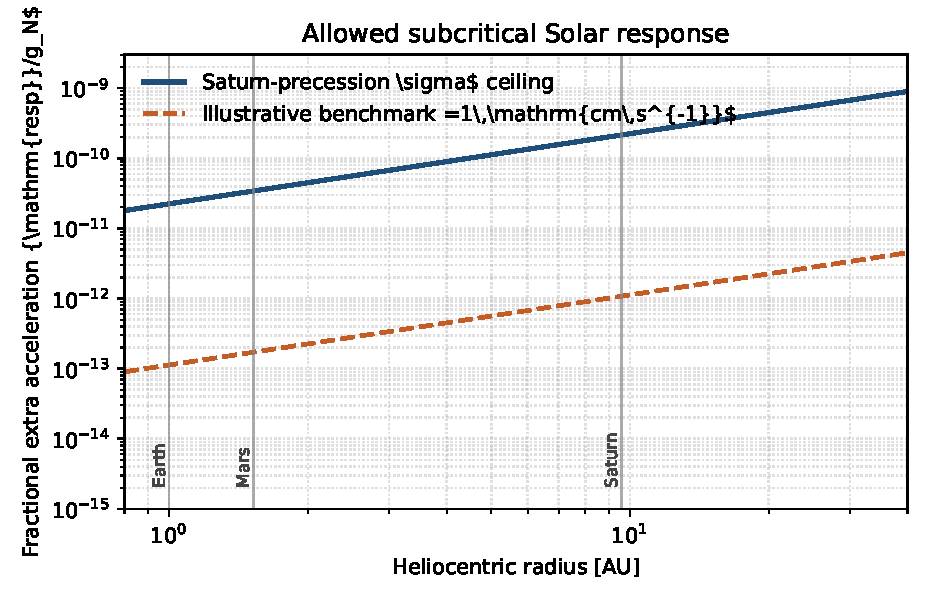
\includegraphics[width=0.86\textwidth]{paper4_solar_response_bounds.pdf}
\caption{Fractional Solar response $\epsilon(r)=V_\odot^{2}r/(GM_\odot)$.
The upper curve uses the Saturn-perihelion one-sigma ceiling~\eqref{eq:Vbound}.
The dashed curve is the illustrative benchmark $V_\odot=1\,\mathrm{cm\,s^{-1}}$.
Outer heliocentric radii are relatively more constraining.}
\label{fig:solarbound}
\end{figure}

\section{Cassini: dynamics versus \texorpdfstring{$\gamma$}{gamma}}
\label{sec:cassini}
Cassini supplies two distinct classes of information that should not be conflated.

\paragraph{Saturn dynamics.}
The long Cassini tracking arc strongly improved Saturn's ephemeris and is already a major reason Saturn provides a stringent outer-planet test~\cite{Pitjeva2013}.
The dynamical bound above therefore already incorporates Cassini-era information through the planetary ephemeris solution.

\paragraph{Solar-conjunction time delay.}
The 2002 Cassini solar-conjunction experiment measured
\begin{equation}
\gamma=1+(2.1\pm2.3)\times10^{-5},
\end{equation}
consistent with general relativity~\cite{Bertotti2003}.
This constrains the relation between the weak-field metric potentials governing matter dynamics and light propagation.
The present response model specifies an additional nonrelativistic acceleration but has not yet supplied a unique relativistic metric closure.
It would therefore be incorrect to convert the Cassini $\gamma$ uncertainty directly into a bound on $V_\odot$ without an additional assumption.
Any relativistic completion must preserve the Cassini bound on gravitational slip; that is a consistency requirement, not a derivation of $\gamma$.

\paragraph{Saturn as a source.}
The same logic can in principle be applied to a response sourced by Saturn itself, $g_{\mathrm{resp}}^{(\mathrm{Sat})}=V_{\mathrm{Sat}}^{2}/s$.
Cassini Grand Finale gravity solutions are optimized for the planet's monopole, zonal harmonics, tides, rings, and spacecraft systematics~\cite{Iess2019}, not for an added logarithmic monopole.
A robust bound on $V_{\mathrm{Sat}}$ therefore requires a dedicated re-fit; we do not manufacture one from published harmonic uncertainties.

\section{Logical status of the results}
\label{sec:status}
\begin{center}
\small
\begin{tabular}{@{}p{0.38\linewidth}p{0.54\linewidth}@{}}
\toprule
\textbf{Quantity / claim} & \textbf{Status}\\
\midrule
$g_{\mathrm{resp}}=CQ/r$ far-field shape & Inherited from~\cite{boyd2026galactic} (Lean-checked there).\\
$g_{\mathrm{resp}}=V_\odot^{2}/r$, $\epsilon(r)$, $M_{\mathrm{resp}}$ & Specialization / definitions (Lean).\\
Gauss reduction to~\eqref{eq:gauss} & Literature hypothesis (Remark~\ref{rem:gauss}).\\
Kepler $\int\cos f/(1+e\cos f)\,df$ & Literature hypothesis (Lean \texttt{literature\_kepler\_cos\_integral}).\\
Perihelion formula~\eqref{eq:Delta-varpi} and circular limit & Proposition~\ref{prop:perihelion} / Cor.~\ref{cor:circular} (Lean algebra on that integrand).\\
Saturn $\dot\varpi$ uncertainty $\to V_\odot$ ceiling & Observational translation of~\cite{Pitjeva2013}.\\
Enclosed-mass consistency scale & Observational consistency check, profile-dependent.\\
Benchmark $V_\odot=0.01\,\mathrm{m\,s^{-1}}$ & Illustrative point inside the allowed window.\\
Cassini $\gamma$ & Independent relativistic consistency condition~\cite{Bertotti2003}.\\
Saturn-centric $V_{\mathrm{Sat}}$ bound & Deferred; dedicated re-fit required.\\
\bottomrule
\end{tabular}
\end{center}

\section{Conclusion}
\label{sec:conclusion}
The long-range response law can be carried into the Solar System without predicting an already-excluded galactic-strength anomaly.
The Saturn perihelion uncertainty implies $V_\odot<0.141\,\mathrm{m\,s^{-1}}$ for the model-specific $1/r$ force, while existing enclosed-mass analyses suggest a comparable tighter consistency scale near $0.086\,\mathrm{m\,s^{-1}}$.
A nonzero benchmark $V_\odot=0.01\,\mathrm{m\,s^{-1}}$ produces effects below current bounds.
Cassini's solar-conjunction test remains an independent requirement on any relativistic completion, not a direct measurement of the nonrelativistic response amplitude.
The paper therefore establishes an observationally allowed subcritical window and a concrete program for closing it: include $V_\odot^{2}/r$ explicitly in modern ephemeris fits, and likewise test $V_{\mathrm{Sat}}^{2}/s$ in a Cassini Grand Finale re-reduction.

\bibliographystyle{plain}
\bibliography{paper_4_refs}
\end{document}
